\documentclass{standalone}
\usepackage{tikz}
\usetikzlibrary{positioning, shapes.misc}

\begin{document}

\begin{tikzpicture}

% Placeholder image
\node[inner sep=0, outer sep=0] (image) at (0,0) {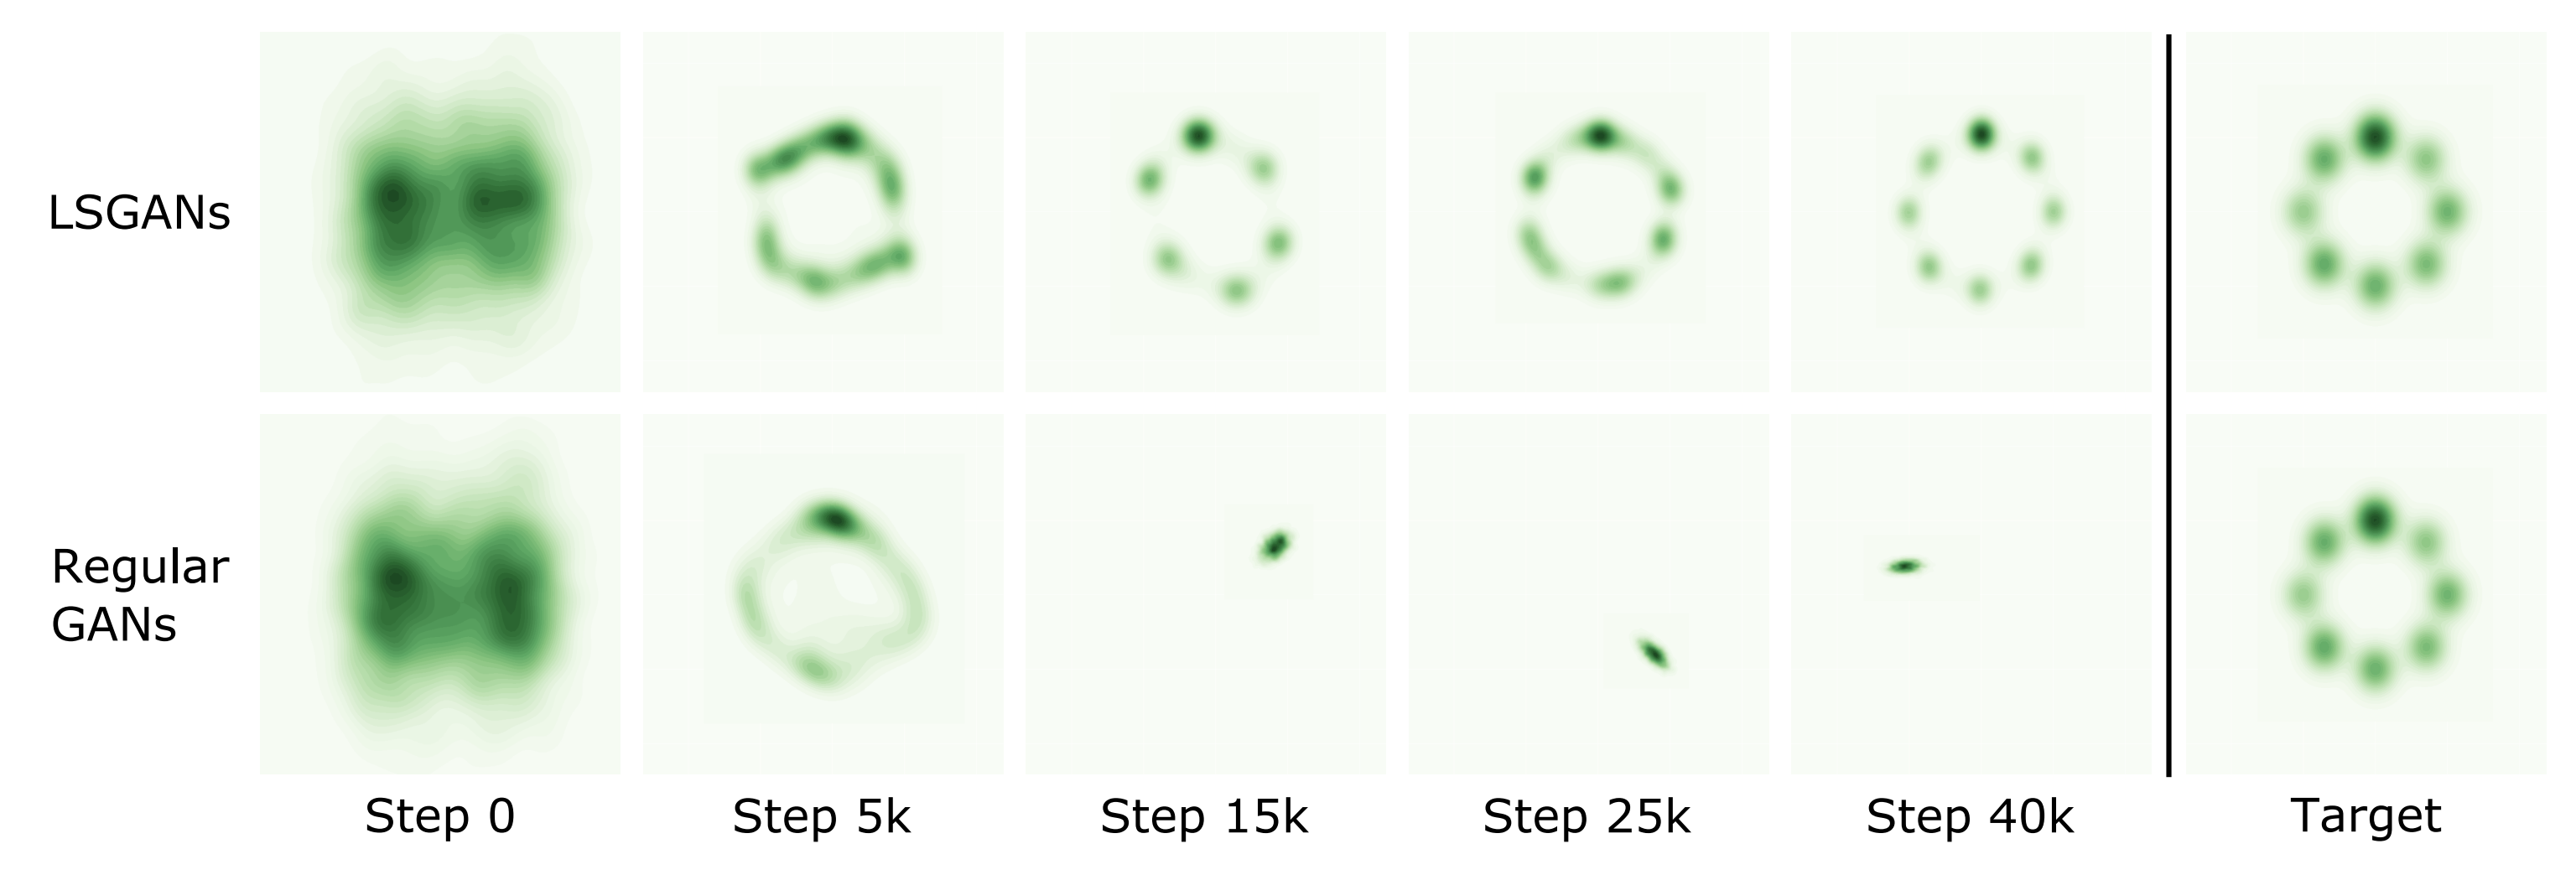
\includegraphics[width=20cm,height=6cm]{tikz/chapter9 - LSGAN.png}};
\node[fill=white, xshift=-6.5cm, yshift=-2.65cm] {\large Step 0};
\node[fill=white, xshift=-3.6cm, yshift=-2.65cm] {\large Step 5K};
\node[fill=white, xshift=-0.6cm, yshift=-2.65cm] {\large Step 15K};
\node[fill=white, xshift=2.3cm, yshift=-2.65cm] {\large Step 25K};
\node[fill=white, xshift=5.3cm, yshift=-2.65cm] {\large Step 40K};
\node[fill=white, xshift=8.4cm, yshift=-2.65cm] {\large Target};


\node[fill=white, xshift=-9cm, yshift=1.5cm] {\large LSGANs};
\node[fill=white, xshift=-9cm, yshift=-0.95cm] {\large Regular};
\node[fill=white, xshift=-9cm, yshift=-1.45cm] {\large  GANs};
\end{tikzpicture}

\end{document}